\scanpage{13}\mspage{6}
\uline{NB} L'ensemble produit à $4$ éléments
\[
\deleted{\unsure{\underline\omega_Q\times}}C\times D
\]
peut s'identifier à l'ensemble quotient $\mathcal{R}/\underline a$ des repères du carré $Q$, modulo antipodisme
\[
C\times D\simeq \mathcal{R}/\underline a\qquad \mathcal{R}=\mathrm{Rep}(Q)\simeq\mathrm{Rep}(Q^{\unsure{o|0|\circ}})
\]
\figure{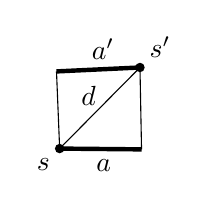
\begin{tikzpicture}[x=1cm,y=1cm]
\draw (0,.05)--(-.04,1.03) (1.04,.04)--(1.02,1.08);
\draw[line width=1.6pt](-.04,1.03)--(1.02,1.08) (0,.05)--(1.04,.04);
\draw (0,.05)--(1.02,1.08);
\fill (0,.05) circle (.06) (1.02,1.08) circle (.06);
\node[below left] at (0,.05){$s$}; \node[above right] at (1.02,1.08){$s'$};
\node[above] at (.55,1.06){$a'$}; \node[below] at (.56,.04){$a$};
\node[above left,inner sep=1pt] at (.50,.56){$d$};
\end{tikzpicture}}
tandis que $\underline\omega_Q$ s'identifie à \deleted{l'ensemble} un ensemble de deux parties de $\mathcal{R}$ (``$\mathcal{R}^+$'' et ``$\mathcal{R}^-$'') complémentaires l'une de l'autre, et stables chacune par l'antipodisme $\underline a$ (qui conserve l'orientation), ce qui fait que le choix d'un élément de $\mathcal{R}/\underline a$ définit canoniquement une orientation de $Q$, \deleted{\unsure{i.e.}} i.e. un des deux \deleted{\unsure{sous-ens.}} ens. de repères $\mathcal{R}',\mathcal{R}''$. Pour vérifier \deleted{que} si cette description d'une isom. $C\wedge D\simeq\underline\omega_Q$ i.e. d'une relation $\underline\omega_Q\wedge C\wedge D\simeq1$ correspond à $(*)$ \deleted{\unsure{$\varpi$}$\wedge c\wedge d=\unsure{0|1}$}, \inserted{$\varpi c d=1$}, il faut expliciter d'abord la convention qui nous \deleted{\unsure{fait|font}} conduit aux plongements
\[
\begin{aligned}
C&\hookrightarrow V_S\setminus\{1,\underline a\}\subset\unsure{\mathfrak{D}|\mathscr{D}},\quad D\hookrightarrow V_A\setminus\{1,\underline a\}\subset\mathfrak{D},\\
&\underline\omega_Q\subset\mathfrak{D}^+\subset\mathfrak{D}.
\end{aligned}
\]
Si $c$ est une \inserted{codiagonale i.e.} paire de côtés opposés du carré, je vais lui associer l'autom \unsure{$j_c$|$J_c$|$\gamma_c$} du carré qui fixe ces deux côtés et qui échange les deux autres i.e. la symétrie p.r. à l'axe transverse. \unsure{Dualement|Idemt|Autrement|De même}, pour une diagonale, je lui associe la symétrie par rapport à cette diagonale. Pour une orientation définie par un repère \deleted{\unsure{ce}}
\figure{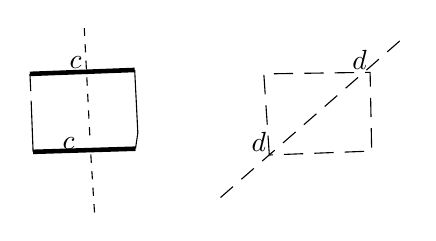
\begin{tikzpicture}[x=1cm,y=1cm]
\draw (0,.06)--(-.025,.71) (-.03,.83)--(-.04,1.05) (1.3,.1)--(1.33,.3)--(1.29,1.1);
\draw[line width=1.65pt](-.04,1.05)--(1.29,1.1) (0,.06)--(1.3,.1);
\draw[dashed](.78,-.71)--(.73,.07) (.72,.27)--(.65,1.63);
\node[above left,inner sep=.5pt] at (.64,1.09){$c$}; \node[above,inner sep=.5pt] at (.45,.07){$c$};
\begin{scope}[xshift=3cm]
\draw[dash pattern=on 7pt off 4pt](0,.02)--(-.07,1.05)--(1.28,1.07)--(1.30,.07)--(0,.02);
\draw[dash pattern=on 6pt off 4pt](-.62,-.52)--(1.75,1.55);
\node[above left,inner sep=1pt] at (0,.02){$d$}; \node[above left,inner sep=1pt] at (1.28,1.07){$d$};
\end{scope}
\end{tikzpicture}}
% archive sheet number: 12
